
\chapter{\IfLanguageName{dutch}{Proof of concept}{Proof of concept}}%
\label{ch:poc}

\section{inleiding}%
Aan de hand van de shortlist die opgemaakt is komt er voor elke geselecteerde managementplatform een proof of concept. Hierbij wordt er gekeken hoe de nodige functionaliteiten werken en toegepast kunnen worden in het systeem.
Belangrijk om te weten is dat de proof of concept niet de volledige functionaliteit van het managementplatform zal testen. Het doel is om een goed beeld te krijgen van de mogelijkheden en hoe deze kunnen worden toegepast binnen de infrastructuur van Excentis. 
We verdelen alle virtual managementplatformen in hun eigen subsecties. In deze subsecties worden dan de vooropgestelde testen op uitgevoerd.
\section{Proxmox VE}%

Voor deze virtual managementplatform wordt er Proxmox VE 8.4 gebruikt. Dit is de laatste versie van Proxmox VE die op dit moment beschikbaar is.
\subsection{cluster opstelling in Proxmox VE}
Voor proxmox VE is er gekozen om te werken met 3 fysieke node's. Zoals beschreven op de officiële documentatiepagina van Proxmox~\cite{proxmoxHA} ondersteunt het platform high availability clustering maar moeten er minimaal 3 nodes in de cluster draaien.
Hierbij spreken we over minimaal 50\% van de nodes die moeten draaien om de cluster operationeel te houden. Dit is ook de reden waarom er voor 3 nodes is gekozen. Bij 2 nodes zou er bij een node failure geen quorum zijn en zou de cluster niet meer operationeel zijn.
In de figuur hieronder wordt de opstelling getoont. Elke node heeft zijn unieke naam in de cluster, vaak is dat de hostname zelf.
\begin{figure}[H]
  \centering
  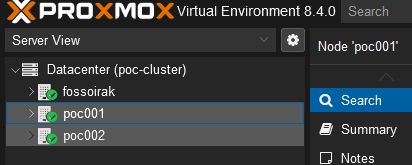
\includegraphics[width=0.85\textwidth]{../poc/cluster-info-prox.png}
  \caption{Clusteropstelling in Proxmox VE}
  \label{fig:cluster-proxmox}
\end{figure}
\subsection{Storage in Proxmox VE}
Proxmox VE ondersteunt verschillende soorten storage. In de proof of concept is er gekozen om te werken met een CEPH storage als distributed storage. Dit is een open-source software-defined storage oplossing die kan worden gebruikt in combinatie met Proxmox VE.
Om deze te configureren moeten er minimaal 3 schijven/partities zijn. Voor deze POC is er besloten om op elke fysieke node een fysieke schijf toe te kennen aan de CEPH storage. Dit zijn 3 willekeurige harde schijven.
Via de GUI kan je via elke node doorklikken naar CEPH hierin moet er dan de schijf worden aangeduid die je wilt gebruiken voor de CEPH storage. Dit kan ook via de command line.

Eenmaal de schijven in elke node te hebben toegevooegd kan je via OSD het overzicht zien.
\begin{figure}[H]
  \centering
  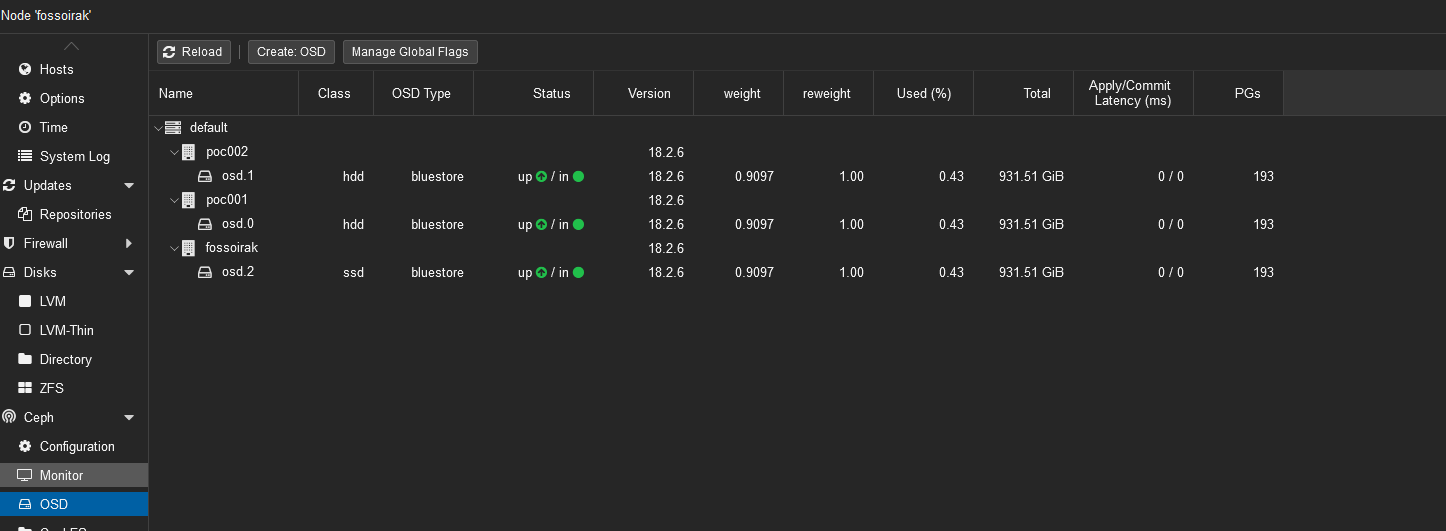
\includegraphics[width=0.85\textwidth]{../poc/ceph-osd-prox.png}
  \caption{CEPH schijven opstelling in Proxmox VE}
  \label{fig:osd-ceph-proxmox}
\end{figure}

Nu kan er een pool aangemaakt worden voor de CEPH storage. Hierin wordt het belangrijskte deel van de CEPH configuratie gedaan.
Je geeft aan hoeveel schijven er in de pool moeten zitten. Minimaal is dit hier 3 aangezien we weer met het HA systeem zitten. Om de HA regels te volgen is het ook essentieel dat er op elke fysieke node een schijf zit voor de pool.
Proxmox VE moet ook weten met CEPH wat de minimaal aantal schijven moeten zijn die operationeel moeten zijn om de pool te kunnen gebruiken. Voor deze POC wordt dit opgesteld op 2. Dit is ook de reden waarom er met 3 fysieke nodes is gewerkt. Bij een node failure kan de pool nog steeds gebruikt worden.
De Crush rule in de configuratie is ook belangrijk. Dit is de manier waarop de data verdeeld wordt over de verschillende schijven. Hierin kan je ook aangeven dat er een replica van de data moet worden gemaakt op een andere node. Bij een node failure kan de data nog steeds worden benaderd via de andere nodes.
Merk op dat de pool naam cepha is.
\begin{figure}[H]
  \centering
  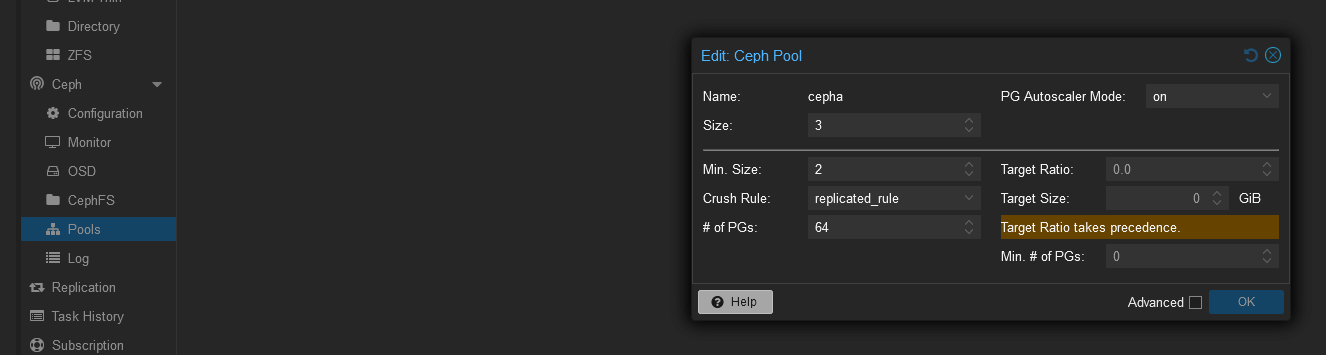
\includegraphics[width=0.85\textwidth]{../poc/ceph-pool-prox.png}
  \caption{Pool opstelling van CEPH in Proxmox VE}
  \label{fig:ceph-pool-prox}
\end{figure}

Eenmaal aangemaakt kan er een virtuele machine worden aangemakt. Deze virtuele machine zal gedraaid worden met ubuntu 22.04.
De meeste instellingen kunnen helemaal naar keuze worden ingesteld en is voor de rest buiten de scope van deze bachelorproef. De belangrijkste instellingen zijn die rond de storage.
Tijdens het configureren van de virtuele machine kan je de schijf kiezen die je wilt gebruiken. Hierin kan je ook de pool selecteren die je hebt aangemaakt. Dit is de pool cepha.
Merk verder op dat er al een optie is voor SAN isci met truenas~\autocite{truenas} . Deze optie mag tijdelijk genegeerd worden.
Als alles goed verloopt kan je op alle 3 de nodes naar keuze een virtuele machine aanmaken en krijgen zij allemaal dezelfde optie op als disk cepha te gebruiken.
\begin{figure}[H]
  \centering
  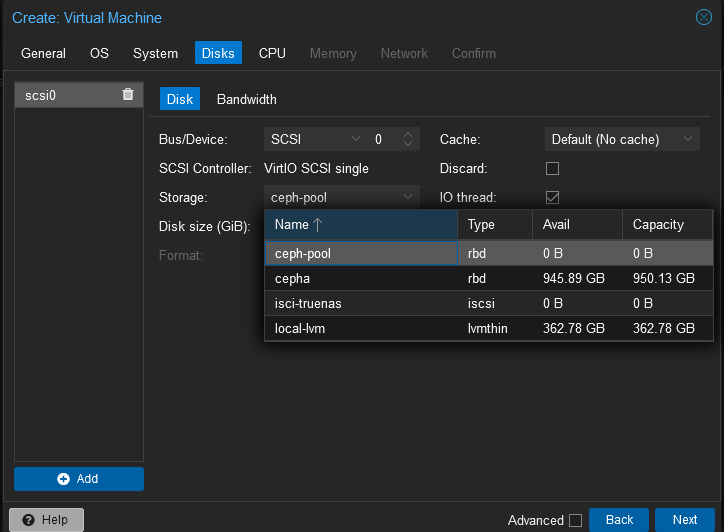
\includegraphics[width=0.85\textwidth]{../poc/vm-storage-prox.png}
  \caption{VM configuratie met correcte disk in Proxmox VE}
  \label{fig:vm-storage-proxmox}
\end{figure}

De virtuele machine is nu aangemaakt op de node fossoirak.
Ter controle kan er in de GUI onder Datacenter bij de optie CEPH gekeken worden of alle schijven en nodes die de CEPH pool draaien healthy zijn.
Als er geen rode kruisjes staan bij de schijven en nodes is alles perfect geconfigureerd.
\begin{figure}[H]
  \centering
  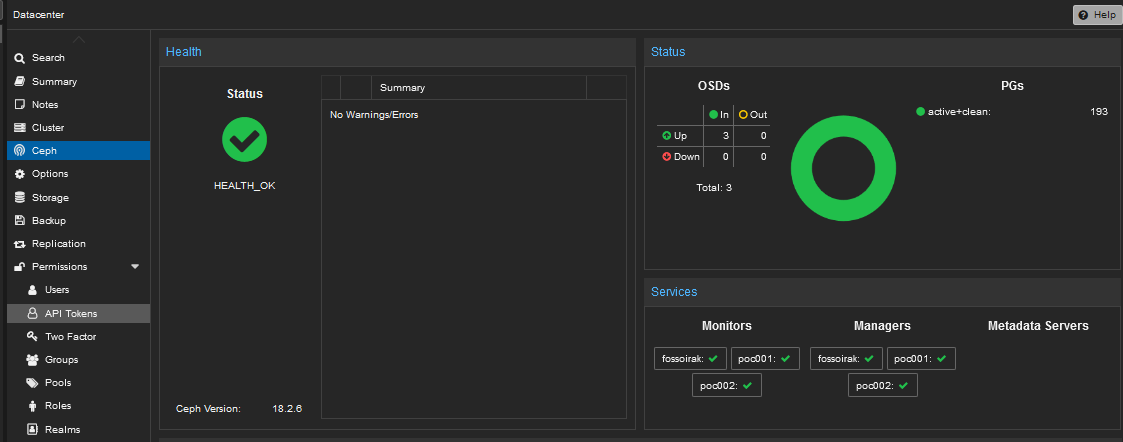
\includegraphics[width=0.85\textwidth]{../poc/ceph-healthy-prox.png}
  \caption{de gezondheid van CEPH  in Proxmox VE}
  \label{fig:ceph-healthy-prox}
\end{figure}

Hierna kan er een HA test uitgevoerd worden. Dit wordt later besproken.
Tijdens het werken met Proxmox VE valt er op dat Proxmox VE automatisch een direct attach storage mount aanmaakt voor te gebruiken. Deze wordt gemount als een directory met als naam local.
Dit toont aan dat Proxmox VE standaard een integratie bied met DAS. In deze situatie draait het direct op de schijf waar de Proxmox VE zelf op draait.
\begin{figure}[H]
  \centering
  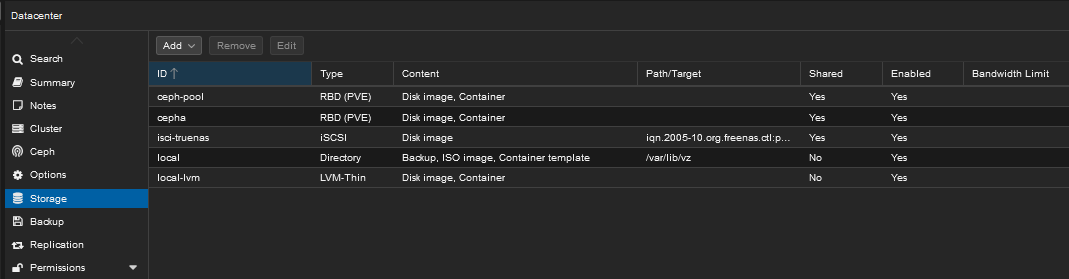
\includegraphics[width=0.85\textwidth]{../poc/das-proxmox.png}
  \caption{direct attach storage in Proxmox VE}
  \label{fig:das-prox}
\end{figure}


Nu we weten dat CEPH goed werkt moet er gekeken worden naar de SAN configuratie met ISCSI.
Er is een bestaande Truenas ~\autocite{truenas} server die al draait in de omgeving. Hierop draait een block storage waar ISCI is geconfigureerd.
Onder het tabje storage  bij Datacenter kan er zeer eenvoudig een iSCSI target worden aangemaakt bij Add.
Via de opties in het menu moet er een correct ID als naam worden gegeven en via portal het correct IP adres van de truenas service.
Omdat er gewerkt wordt met een SAN princiepe staat het default bij de optie node in de configuratie op all nodes. Dit is ook de bedoeling aangezien we met een HA cluster werken.
De configuratie van ISCI op truenas is buiten de scope van deze bachelorproef.
\begin{figure}[H]
  \centering
  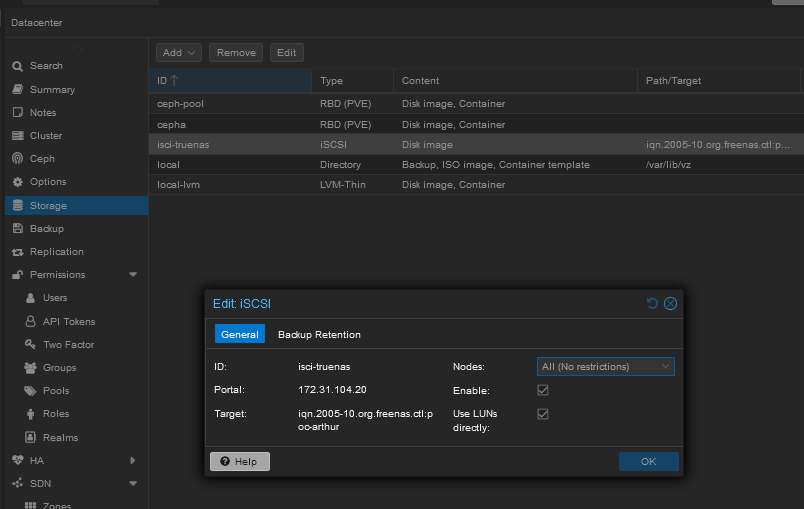
\includegraphics[width=0.85\textwidth]{../poc/iscsi-prox.png}
  \caption{storage area network met ISCI in Proxmox VE}
  \label{fig:iscsi-SAN}
\end{figure}
Nu zal er een extra  optie bijgekomen zijn in de GUI onder het tabje storage bij datacenter. Hier in het voorbeeld wordt het al naam isci-truenas gegeven.
Nu maken we een 2de virtuele machine aan met dezelfde configuratie als de eerste virtuele machine maar met een andere disk. Er wordt nu gekozen voor de isci-truenas disk.
\begin{figure}[H]
  \centering
  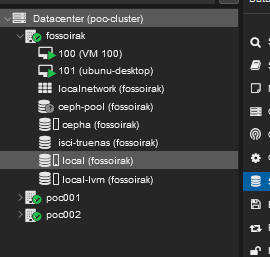
\includegraphics[width=0.85\textwidth]{../poc/vm-lijst-prox.png}
  \caption{Lijst van de 2 virtuele machines in Proxmox VE}
  \label{fig:vm-lijst}
\end{figure}
Aangezien een SAN princiepe via een vebrinding werkt op het netwerk is de storage de zwakste schakel in een high availability cluster
\subsection{High Availability in Proxmox VE}

Eenmaal de storage in orde is voor de virtuele machines kan er een HA configuratie worden aangemaakt. 
Onder Datancenter HA kan je een group aanmaken. Hierin beschrijf je alle 3 de fysieke nodes die in de cluster zitten. Vervolgens geven we de groep een logische naam. In dit geval is het de naam ha-pool.
\begin{figure}[H]
  \centering
  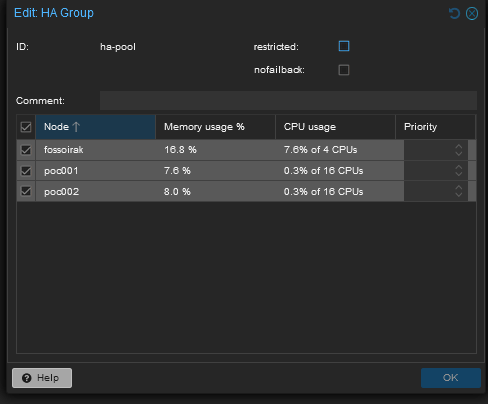
\includegraphics[width=0.85\textwidth]{../poc/ha-group.png}
  \caption{high Availability group in Proxmox VE}
  \label{fig:ha-group}
\end{figure}
Nu voegen we de 2 virtuele machines toe aan de HA groep. Dit wordt gedaan via de HA section in datancer.
Bij Max restart en max relocate zet je aan hoeveel keer de virtuele machine opnieuw mogen worden opgestart of verplaatst naar een andere node. In dit geval moet dit groter zijn dan 0.
\begin{figure}[H]
  \centering
  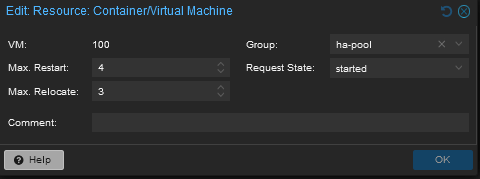
\includegraphics[width=0.85\textwidth]{../poc/vm-ha.png}
  \caption{High Availability vm toevoegen in Proxmox VE}
  \label{fig:ha-vm}
\end{figure}
Als beide virtuele machines zijn toegevoegd aan de HA groep kan je de HA configuratie testen.

Om HA te testen in combinatie met beide storage systemen zal er een netwerk probleem worden gesimuleerd.
Alle virtuele machines draaien nu op node 001
Op de fysieke node poc001 zal de internet kabel worden uitgetrokken. Hierna kijken we hoelang het duurt vooraleer de virtuele machines opnieuw worden opgestart op een andere node, meer bepaald ook op welke node specifiek.

In de figuur hieronder kan er duidelijk gezien worden dat de virtuele machines volledig van cold mode moeten opstarten. Dit is een andere situatie dan wanneer er een migratie gedaan wordt. Dan wordt live de virtuele machine van de ene node naar de andere gemigreert zonder echte downtime.
Het systeem in Proxmox VE is nu zo ingesteld dat bij een echte failover de schade van downtime relatief beperkt blijft. Dit staat uiteraard los van data verlies die kan optreden bij een failover.
\begin{figure}[H]
  \centering
  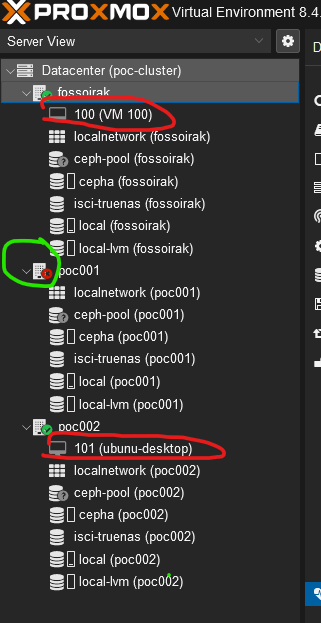
\includegraphics[width=0.85\textwidth]{../poc/failover-prox.png}
  \caption{failover node virtuale machines herstellen in HA in Proxmox VE}
  \label{fig:failover-vm}
\end{figure}

Vanaf de connectie van poc001 verboken is met de nadere nodes duurt het ongeveer 30-60 seconden vooraleer de virtuele machines opnieuw worden opgestart op een andere node. Dit is ook de tijd die nodig is om de heartbeat van de cluster te verliezen.
Hierbij kunenn we vanuit gaan dat de defautl healthy check van de cluster en zijn nodes ook rond deze tijdsduur ligt. Beide virtuele machines worden opnieuw opgestart op de node foissarak en poc 002. 
Aangezien beide virtuele machines dezelfde HA group hebben, krijgen ze ook dezelfde prioriteit.

Merk op dat zowel de virtuele machine met een SAN als de virtuele machine met een distributed storage opnieuw worden opgestart op de node foissarak. Dit toont aan dat Proxmox VE goed werkt met beide storage systemen, zeker met failover situaties.


\subsection{Virtuele machines migraties in Proxmox VE}
In het het werkveld komt het geregeld voor dat een node een gepland onderhoud heeft. Dit kan zijn dat er een update moet worden uitgevoerd of dat er hardware moet worden vervangen.
Bij deze is het gewenst om te weten of er een mogelijkheid is om de virtuele machines te migreren naar een andere node zonder dat er downtime/minimale downtime is.
Via de GUI in Proxmox VE kan je heel eenvoudig een virtuele machine migreren via de migration optie rechts boven als er een virtuele machine geselecteerd is.
\begin{figure}[H]
  \centering
  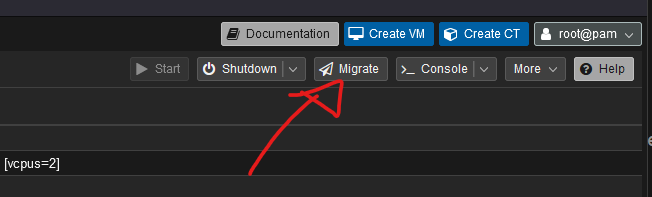
\includegraphics[width=0.85\textwidth]{../poc/vm-migratie-prox.png}
  \caption{migratie virtuele machine in Proxmox VE}
  \label{fig:migratie-vm}
\end{figure}
Tijdens het migreren van de virtuele machine blijft de console open staan van de virtuele machine. Hierbij is er een zeer korte freeze in het beeld waarna de activiteiten in de vm weer verder werken. Het totale proces voor beide virtuele machines individueel was onegveer 30 seconden.
Hieruit kan er bekeken worden dat de downtime bij migratie zo goed als minimaal is, wat ideaal is voor het offline brengen van een node voor bijvoorbeeld een gepland onderhoud.


\subsection{Hot swapping fysieke disks in Proxmox VE}
Proxmox VE bied ook hot swapping aan van de fysieke disks. 
Voor deze test is er een fysieke disk voor node poc002 toegevoegd.
\begin{figure}[H]
  \centering
  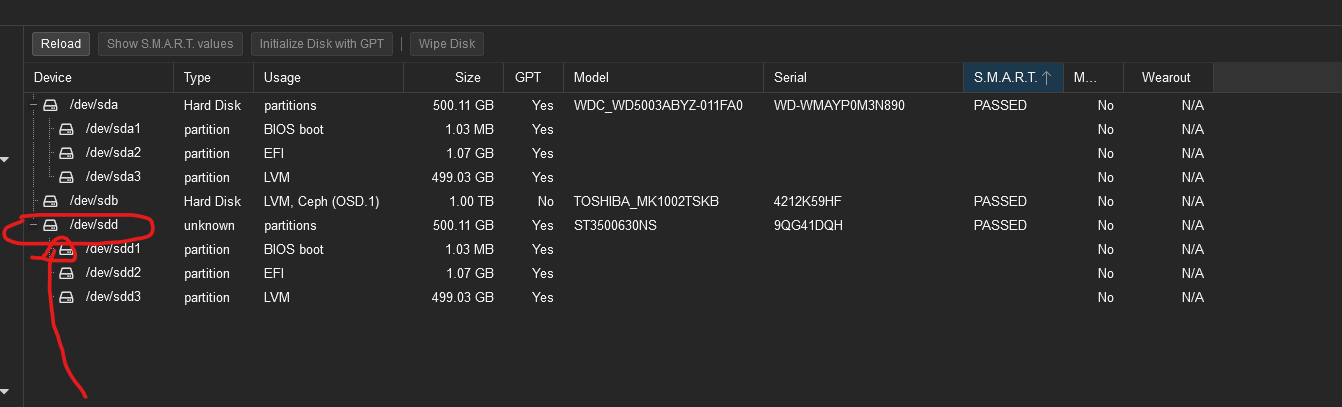
\includegraphics[width=0.85\textwidth]{../poc/hot-disk-prox.png}
  \caption{hot disk swap in Proxmox VE}
  \label{fig:hotdisk-swap}
\end{figure}
Deze noemt sdb. Eenmaal dat deze disk is toegevoegd zou de disk moeten kunnen verwijderd worden en vervangen worden door een andere zonder dat de node poc002 offline moet worden gehaald.
Dit wordt live getest tijden het draaien. Op deze disk draait momenteel niks. Dit is belangrijk aangezien we het vervangen van een disk simuleren. De data zou normaal op voorhand moeten verwijderd zijn van de disk.

We voegen de nieuwe disk toe in de plaats van de andere en merken direct na 15 seconden dit op.
\begin{figure}[H]
  \centering
  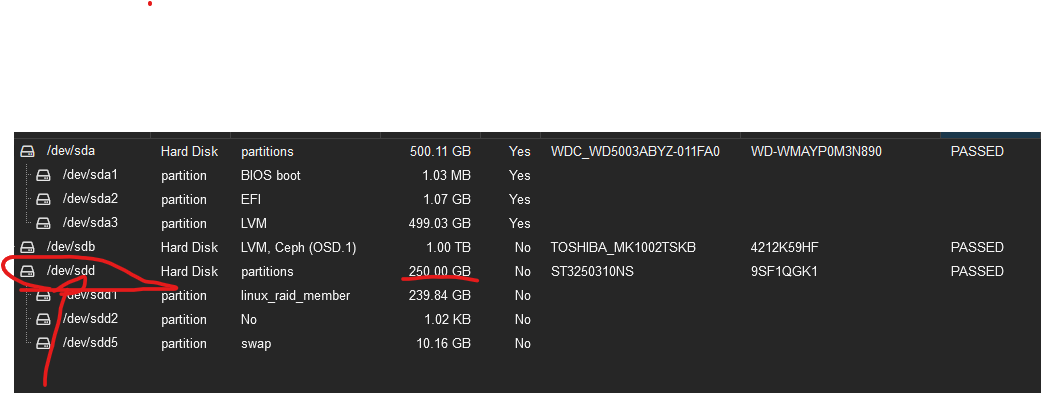
\includegraphics[width=0.85\textwidth]{../poc/hot-disktwee-prox.png}
  \caption{hot disk swap in Proxmox VE}
  \label{fig:hotdiskvervangen-swap}
\end{figure}

We zien dat dit duidelijk een andere disk is met nu een grote van 250 GB. Hiervoor was dat 500 GB.